% Options for packages loaded elsewhere
\PassOptionsToPackage{unicode}{hyperref}
\PassOptionsToPackage{hyphens}{url}
\PassOptionsToPackage{dvipsnames,svgnames*,x11names*}{xcolor}
%
\documentclass[
  11pt,
]{article}
\usepackage[]{mathpazo}
\usepackage{amsmath}
\usepackage{ifxetex,ifluatex}
\ifnum 0\ifxetex 1\fi\ifluatex 1\fi=0 % if pdftex
  \usepackage[T1]{fontenc}
  \usepackage[utf8]{inputenc}
  \usepackage{textcomp} % provide euro and other symbols
  \usepackage{amssymb}
\else % if luatex or xetex
  \usepackage{unicode-math}
  \defaultfontfeatures{Scale=MatchLowercase}
  \defaultfontfeatures[\rmfamily]{Ligatures=TeX,Scale=1}
\fi
% Use upquote if available, for straight quotes in verbatim environments
\IfFileExists{upquote.sty}{\usepackage{upquote}}{}
\IfFileExists{microtype.sty}{% use microtype if available
  \usepackage[]{microtype}
  \UseMicrotypeSet[protrusion]{basicmath} % disable protrusion for tt fonts
}{}
\usepackage{xcolor}
\IfFileExists{xurl.sty}{\usepackage{xurl}}{} % add URL line breaks if available
\IfFileExists{bookmark.sty}{\usepackage{bookmark}}{\usepackage{hyperref}}
\hypersetup{
  pdftitle={Making Migration Sexy: Immigrants in Same-Sex Couples in the United States},
  pdfauthor={Nathan I. Hoffmann, Department of Sociology, University of California, Los Angeles; Kristopher Velasco, Department of Sociology, University of Texas at Austin},
  pdfkeywords={immigration, same-sex couples, LGBTQ policy},
  colorlinks=true,
  linkcolor=blue,
  filecolor=Maroon,
  citecolor=Blue,
  urlcolor=Blue,
  pdfcreator={LaTeX via pandoc}}
\urlstyle{same} % disable monospaced font for URLs
\usepackage[margin=1in]{geometry}
\usepackage{longtable,booktabs}
\usepackage{calc} % for calculating minipage widths
% Correct order of tables after \paragraph or \subparagraph
\usepackage{etoolbox}
\makeatletter
\patchcmd\longtable{\par}{\if@noskipsec\mbox{}\fi\par}{}{}
\makeatother
% Allow footnotes in longtable head/foot
\IfFileExists{footnotehyper.sty}{\usepackage{footnotehyper}}{\usepackage{footnote}}
\makesavenoteenv{longtable}
\usepackage{graphicx}
\makeatletter
\def\maxwidth{\ifdim\Gin@nat@width>\linewidth\linewidth\else\Gin@nat@width\fi}
\def\maxheight{\ifdim\Gin@nat@height>\textheight\textheight\else\Gin@nat@height\fi}
\makeatother
% Scale images if necessary, so that they will not overflow the page
% margins by default, and it is still possible to overwrite the defaults
% using explicit options in \includegraphics[width, height, ...]{}
\setkeys{Gin}{width=\maxwidth,height=\maxheight,keepaspectratio}
% Set default figure placement to htbp
\makeatletter
\def\fps@figure{htbp}
\makeatother
\setlength{\emergencystretch}{3em} % prevent overfull lines
\providecommand{\tightlist}{%
  \setlength{\itemsep}{0pt}\setlength{\parskip}{0pt}}
\setcounter{secnumdepth}{-\maxdimen} % remove section numbering
\usepackage{fancyhdr}
\pagestyle{fancy}
\setlength{\headheight}{13.6pt}
\rhead{\textit{Hoffmann and Velasco}}
\usepackage{booktabs}
\usepackage{longtable}
\usepackage{array}
\usepackage{multirow}
\usepackage{wrapfig}
\usepackage{float}
\usepackage{colortbl}
\usepackage{pdflscape}
\usepackage{tabu}
\usepackage{threeparttable}
\usepackage{threeparttablex}
\usepackage[normalem]{ulem}
\usepackage{makecell}
\usepackage{xcolor}
\ifluatex
  \usepackage{selnolig}  % disable illegal ligatures
\fi
\newlength{\cslhangindent}
\setlength{\cslhangindent}{1.5em}
\newlength{\csllabelwidth}
\setlength{\csllabelwidth}{3em}
\newenvironment{CSLReferences}[2] % #1 hanging-ident, #2 entry spacing
 {% don't indent paragraphs
  \setlength{\parindent}{0pt}
  % turn on hanging indent if param 1 is 1
  \ifodd #1 \everypar{\setlength{\hangindent}{\cslhangindent}}\ignorespaces\fi
  % set entry spacing
  \ifnum #2 > 0
  \setlength{\parskip}{#2\baselineskip}
  \fi
 }%
 {}
\usepackage{calc}
\newcommand{\CSLBlock}[1]{#1\hfill\break}
\newcommand{\CSLLeftMargin}[1]{\parbox[t]{\csllabelwidth}{#1}}
\newcommand{\CSLRightInline}[1]{\parbox[t]{\linewidth - \csllabelwidth}{#1}\break}
\newcommand{\CSLIndent}[1]{\hspace{\cslhangindent}#1}

\title{Making Migration Sexy: Immigrants in Same-Sex Couples in the United States}
\author{Nathan I. Hoffmann, Department of Sociology, University of California, Los Angeles \and Kristopher Velasco, Department of Sociology, University of Texas at Austin}
\date{January 31, 2021}

\begin{document}
\maketitle
\begin{abstract}
As they gain greater social acceptance and new rights, numbers of same-sex couples in the United States are increasing, yet few demographers have studied immigrants in same-sex couples. Using the American Community Survey from 2008 to 2019, this study compares same-sex couples including at least one immigrant to corresponding different-sex couples in order to characterize and assess the scale of sexual migration to the U.S. Moreover, we evaluate how the policy environment related to same-sex couples shapes migratory patterns. We find that same-sex couples generally have higher incomes and come from countries with smaller wage and unemployment differentials with the U.S. Moreover, LGBT policy in country of origin and U.S. state are significantly associated with their migratory patterns. Our findings put into question predominant models of migration that emphasize economic and network effects, suggesting the importance of considering political and lifestyle motivations.
\end{abstract}

\hypertarget{introduction}{%
\section{Introduction}\label{introduction}}

In 2013, the U.S. Supreme Court made a landmark decision overturning the Defense of Marriage Act. This decision reverberated across society. One important outcome was making immigration by same-sex couples more accessible. While numbers of different-sex couples including immigrants increased by 13 percent from 2013 to 2019 (from 8.4 million to 9.5 million), those of immigrant same-sex couples grew from 62 thousand to 108 thousand in the same period, an increase of 75 percent (\protect\hyperlink{ref-u.s.censusbureau_2020}{U.S. Census Bureau 2020}). Indeed, this time period represents an important moment in which policies governing same-sex couples, both in the U.S. and internationally, are changing rapidly. Surprisingly, however, immigration research has not explicitly analyzed how these changes are influencing the push-and-pull of migration patterns of same-sex couples into the U.S. This is partly due to the fact that conventional migration research focuses on a largely economic, cost-benefit analysis and only recently began to factor in the role of social policies (\protect\hyperlink{ref-fitzgerald_2014}{Fitzgerald, Leblang, and Teets 2014}). Moreover, while gender has been recently recognized as an integral part of the migration process (\protect\hyperlink{ref-lutz_2010}{Lutz 2010}; \protect\hyperlink{ref-hondagneu-sotelo_2012}{Hondagneu-Sotelo 2012}), sexuality receives relatively scant attention. As \protect\hyperlink{ref-carrillo_2018}{Carrillo} (\protect\hyperlink{ref-carrillo_2018}{2018}) demonstrates, however, sexuality is a salient factor determining immigration decisions. We show that differences between immigrants in same-sex couples and those in different-sex couples cannot be explained solely using classic theories of migration; consequently, by not making sexuality an integral part of the research question, this limits our understanding of the full immigration process.

Therefore, for this project, we seek to understand how LGBT policies influence same-sex couples migration patterns. Specifically, do policies at country-of-origin and of residing U.S. state influence migration patterns of same-sex immigrant couples? We integrate two types of data to help answer this question. First, we rely on American Community Survey data for 2008 to 2019, which allows the identification of same-sex couples, immigrant origin, U.S. state of residence, and potentially confounding individual characteristics. Second, we harness original datasets indexing LGBT policy changes in 193 countries and all U.S. states from 1991 to 2019 (Velasco xx). Our analytic strategy proceeds in four parts. First, we compare descriptive statistics of immigrants in same- and different-sex couples, assessing how classic migration variables such as income, education, and family size vary between these groups. Second, we focus on country-of-origin effects. We model the proportion of a given immigrant group constituted by same-sex couples, and how this proportion changes over time in response to the LGBT policy context of the country of origin. Third, in order to assess state effects, we model how the proportion of an immigrant group in a given state changes in response to the changing state LGBT policy context. Lastly, we shift our attention to the individual, assessing how being an immigrant in a same-sex couple, net of other individual factors usually considered in migration analyses, bears upon choice of the state LGBT policy context.

Our research shows that origin country policy matters for levels of immigrants in same-sex couples, but perhaps not in the way scholars would expect. Countries of origin with more LGBT-friendly policies send higher proportions of immigrants in same-sex couples. This implies that these policies may enable LGBT individuals looking to migrate, whereas oppressive policies may hinder such ambitions. Second, we find little role of U.S. state policy at the aggregate level of proportion immigrants in same-sex couples, but at the individual level, we find the expected trend: immigrants in same-sex couples are more likely to live in LGBT-friendly states. This effect is moderated by country-of-origin context, however; immigrants in same-sex couples from countries with LGBT-friendly policies are more likely to live in LGBT-friendly states. We find the opposite trend for immigrants in different-sex couples.

\hypertarget{background-changing-policy-landscape-for-same-sex-immigrant-couples}{%
\section{Background: Changing Policy Landscape for Same-Sex Immigrant Couples}\label{background-changing-policy-landscape-for-same-sex-immigrant-couples}}

The U.S. has undergone significant shifts in the policies governing LGBT populations. Since 2003, the U.S. Supreme Court ruled sodomy laws and the Defense of Marriage Act unconstitutional, legalized same-sex marriages, and curtailed employment discrimination. In response, however, a number of policies hindering LGBT communities were implemented at both the state and federal levels -- such as thinly veiled ``religious freedom'' laws -- on top of existing discriminatory policies like state constitutional bans on marriage equality (\protect\hyperlink{ref-kayak_2018}{\textbf{kayak\_2018?}}). This creates a varied landscape in which state lines may significantly demarcate the types of rights and legal environments LGBT people experience. Now, a burgeoning area of scholarship exists to understand the causes of these transformations (\protect\hyperlink{ref-lax_2009}{Lax and Phillips 2009}; \protect\hyperlink{ref-soule_2004}{Soule 2004}) and, even more recently, their distinct consequences on the lives and well-being of LGBT people (\protect\hyperlink{ref-boertien_2019}{Boertien and Vignoli 2019}; \protect\hyperlink{ref-carpenter_2020}{Carpenter 2020}; \protect\hyperlink{ref-kail_2015}{Kail, Acosta, and Wright 2015}; \protect\hyperlink{ref-levy_2017}{Levy and Levy 2017}).

Though this changing policy landscape effects LGBT populations of all types, particular sub-groups within this broad umbrella are likely to be differentially impacted. Same-sex immigrant couples represent a key group especially vulnerable to recent changes. This is because prior to being able to experience recognized rights like marriage or non-discrimination protections, same-sex immigrant couples must first be able to enter into the U.S. Historically, federal U.S. law hindered same-sex immigrant couples' ability to enter the country due to the government's lack of recognition of their relationship (\protect\hyperlink{ref-humanrightswatch_2006}{Watch 2006}). One of the few mechanisms by which queer migrants could enter into the U.S., then, was through the asylum process -- an invasive process in which migrants needed to ``prove'' their sexual desires (\protect\hyperlink{ref-humanrightswatch_2006}{Watch 2006}). These legal exclusions are commonly reflected within academic scholarship where analyses of domestic LGBT communities assume citizenship and migration research assumes migrants as heterosexual (\protect\hyperlink{ref-luibheid_2008}{E. Luibhéid 2008}). Most academic literature that does acknowledge the realities of queer migrants, therefore, has largely centered on the asylum process -- leaving a very shallow understanding of the factors influencing the migratory patterns of same-sex immigrant couples and how they align or diverge from their heterosexual counterparts.

\begin{figure}
\centering
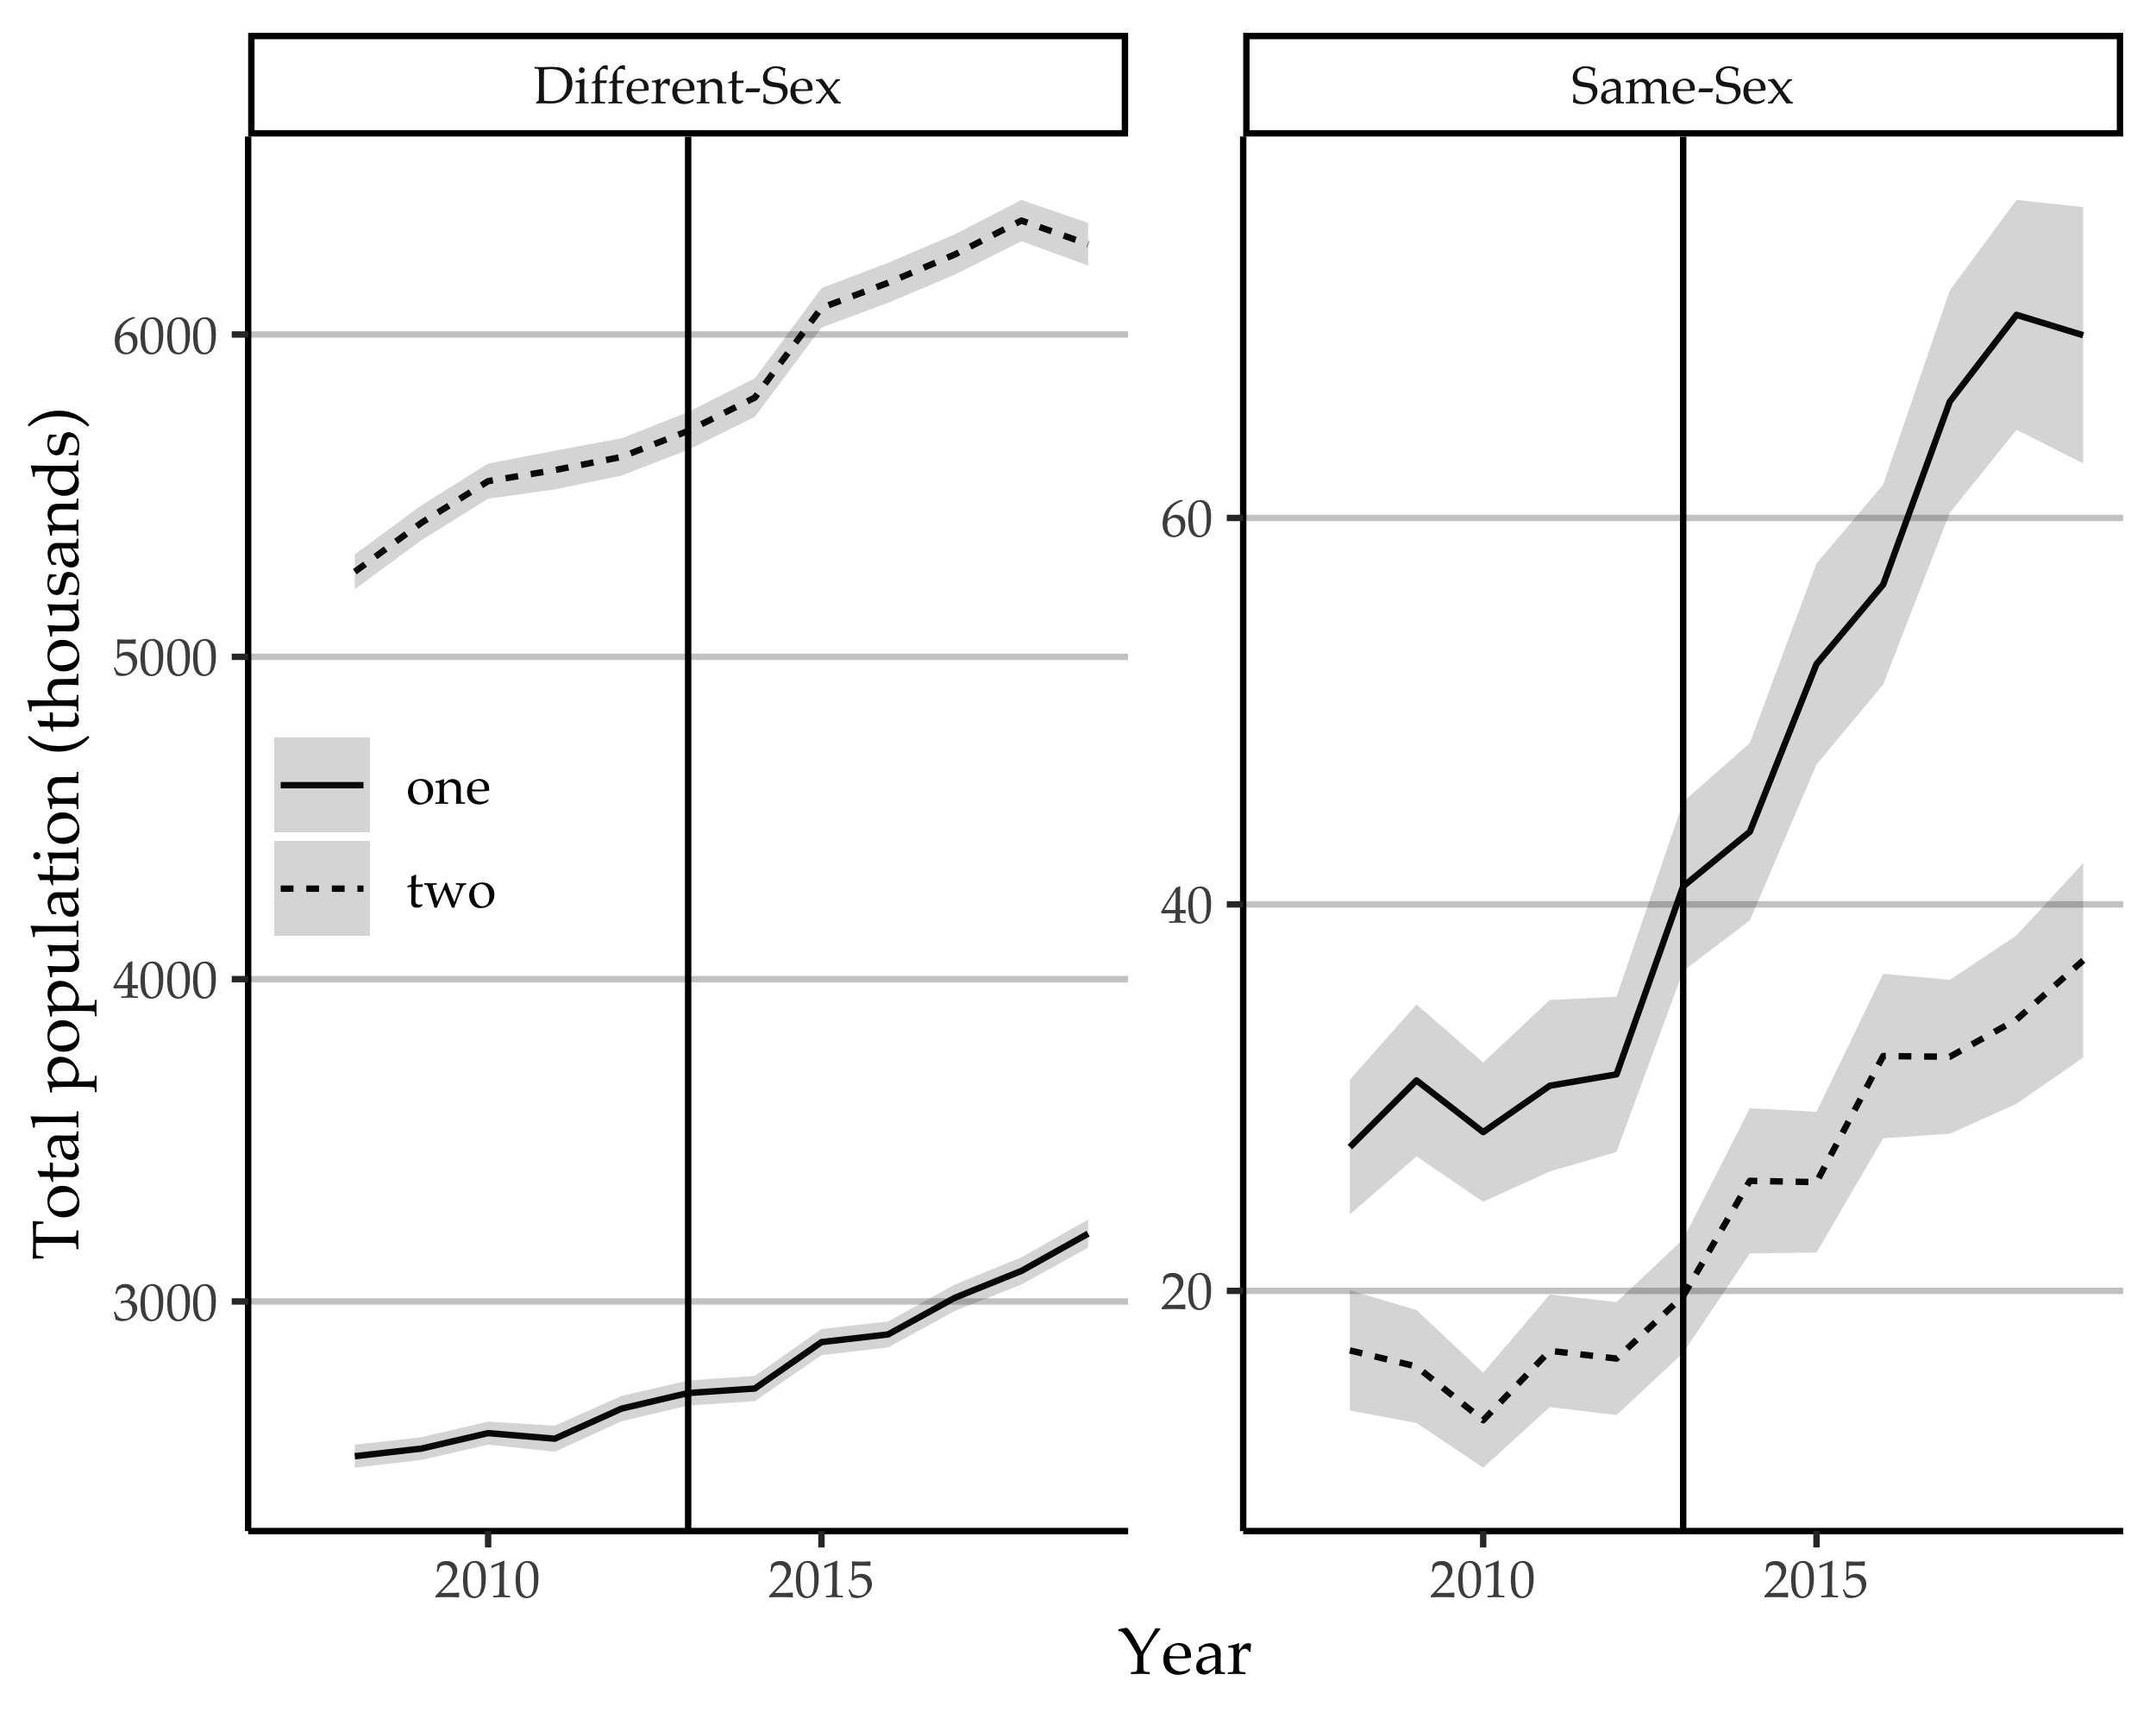
\includegraphics{ssimm_draft_files/figure-latex/total-pop-1.pdf}
\caption{\label{fig:total-pop}Estimated totals of different- and same-sex couples containing one or two immigrants, 2008-2019, with 95\% confidence intervals. Vertical line placed at the year 2013, when DOMA was overturned.}
\end{figure}

This legal environment changed after 2013. The U.S. Supreme Court opinion ruling the Defense of Marriage Act (DOMA) unconstitutional opened the door for more same-sex immigrant couples to enter the U.S. under the same process long-governing different-sex couples. Indeed, as Figure \ref{fig:total-pop} highlights, the number of same-sex immigrant couples in the U.S. grew significantly following this ruling -- especially when compared to different-sex couples. In 2013, there were 62 thousand. By 2019, this grew to 108 thousand. Aside from allowing gay and lesbian families to remain unified, this national opening creates an important moment for the scholarly community as well. Now, more careful investigation into the factors both pushing and pulling same-sex immigrant couples into the U.S. can be done -- beyond idiosyncratic outcomes based on asylum claims. The present research fits squarely within this critical research gap.

\hypertarget{understanding-influences-on-migration-patterns}{%
\section{Understanding Influences on Migration Patterns}\label{understanding-influences-on-migration-patterns}}

\hypertarget{conventional-explanations}{%
\subsection{Conventional Explanations}\label{conventional-explanations}}

Our analysis compares conventional explanations for migration to political ones related to LGBT policy. These conventional explanations are frequently combined in a ``gravity model,'' which Anderson (\protect\hyperlink{ref-anderson_2011}{2011, 134}) describes in general terms: ``A mass of goods or labor or other factors of production supplied at origin \(i\), \(Y_i\), is attracted to a mass of demand for goods or labor at destination \(j\), \(E_j\), but the potential flow is reduced by the distance between them, \(d_{ij}\).'' This model continues to be widely applied to predict large-scale migration (\protect\hyperlink{ref-karemera_2000}{Karemera, Oguledo, and Davis 2000}; \protect\hyperlink{ref-poot_2016}{Poot et al. 2016}).

Neoclassical economic theories motivates the variables to include. Promise of material gain is a frequent motivation to migrate (\protect\hyperlink{ref-hatton_2005a}{Hatton and Williamson 2005}; \protect\hyperlink{ref-todaro_1980}{Todaro 1980}); at the micro level, individuals who stand to gain greater returns to their education are more likely to migrate. At the macro level, neoclassical economics predicts that migrants will follow wage and unemployment differentials across countries. Hence gravity models usually include difference in per capita GDP between sending and receiving countries. These neoclassical theories also posit that migration costs are as important as benefits. A proxy for cost of migration in the gravity model is distance: immigrants are more likely to migrate between proximate countries, especially those that share a border.

Although the traditional gravity model focuses only on distance and economic ``mass,'' in recent years it has been refined with the incorporation of political and cultural variables (\protect\hyperlink{ref-karemera_2000}{Karemera, Oguledo, and Davis 2000}; \protect\hyperlink{ref-fitzgerald_2014}{Fitzgerald, Leblang, and Teets 2014}). Scholars have shown that shared language, colonial history, and democratization matter in the sending country, and immigrant rights matter in the receiving country. However, these models have not yet considered political variables directly related to LGB individuals, or how such policies might affect their migration.

\hypertarget{our-intervention}{%
\subsection{Our Intervention}\label{our-intervention}}

Though migration scholarship typically emphasizes economic considerations, we argue that it is also imperative to take sexuality, and the state's role in governing sexuality, into account for understanding migratory patterns (\protect\hyperlink{ref-carrillo_2018}{Carrillo 2018}; \protect\hyperlink{ref-fitzgerald_2014}{Fitzgerald, Leblang, and Teets 2014}). One reason why this area of research has yet to be fully considered, in addition to previous restrictions outlined, is because the literature largely assumes immigrants as heterosexual or simply neglects to consider them as fully constitutive, diverse sexual beings (\protect\hyperlink{ref-canaday_2009}{Canaday 2009}; \protect\hyperlink{ref-epstein_2014}{Epstein and Carrillo 2014}; \protect\hyperlink{ref-gonzalez-lopez_2005}{González-López 2005}).

Consequently, analyses into how sexuality motivates migratory decisions or how migration reimagines sexual behaviors and understandings are limited (\protect\hyperlink{ref-carrillo_2018}{Carrillo 2018}). Even more limited, are explicit analyses into how policies such as same-sex marriage, hate crime protections, sodomy, and the like, further complicate migration patterns. The nascent scholarship concerning queer migrants that does exist, though, suggests that policy environments are a central concern when making these decisions (\protect\hyperlink{ref-cantu_2009}{Cantú 2009}; \protect\hyperlink{ref-luibheid_2005}{Eithne Luibhéid and Cantú 2005}). Therefore, below, we theorize why LGBT policies at country-of-origin and residing U.S. state influence the push and pull of same-sex couples within the U.S.

Laws governing LGBT communities have significantly transformed. These changes are part of a broader global trend in which LGBT rights are increasingly incorporated within existing human rights frameworks -- pressuring countries to respond in turn (\protect\hyperlink{ref-velasco_2018}{Velasco 2018}). These new dynamics have spurred research into understanding the causes of policy reforms and why countries have taken such varied approaches to enacting reform -- both in expanding rights but also further restricting them (\protect\hyperlink{ref-ayoub_2016}{Ayoub 2016}). Only recently are scholars starting to understand the direct consequences of these changes on the lives of LGBT people (\protect\hyperlink{ref-boertien_2019}{Boertien and Vignoli 2019}; \protect\hyperlink{ref-carpenter_2020}{Carpenter 2020}; \protect\hyperlink{ref-kail_2015}{Kail, Acosta, and Wright 2015}). Though this emerging scholarship focuses largely on health and subjective well-being, particularly concerning marriage laws, there are several reasons why these new realities are likely to shape the migration of same-sex couples.

Sexuality has long factored into migratory decisions. However, as the global awareness of LGBT rights expands, sexuality is increasingly a salient and important factor when deciding to leave one's home country (\protect\hyperlink{ref-mole_2018a}{Mole 2018}; \protect\hyperlink{ref-murray_2016}{Murray 2016}). Part of this is due to international organizations' construction of sexuality as a legitimate basis for leaving. For example, in 2008, the United Nations High Commissioner for Refugees issued a new guidance note for why and how countries should consider sexual orientation and gender identity when granting asylum claims. The note states:

\begin{quote}
``\ldots individuals experience serious human rights abuses and other forms of persecution due to their actual or perceived sexual orientation and/or gender identity. While persecution of Lesbian, Gay, Bisexual, Transgender and Intersex (hereafter ``LGBTI'') individuals and those perceived to be LGBTI is not a new phenomenon, there is greater awareness in many countries of asylum that people fleeing persecution for reasons of their sexual orientation and/or gender identity can qualify as refugees\ldots''
\end{quote}

The note continues to guide various authorities to consider discriminatory domestic policies when evaluating asylum claims as such policies ``can create or contribute to an oppressive atmosphere of intolerance and generate a threat of prosecution,'' (\protect\hyperlink{ref-unhcr_2008}{\textbf{unhcr\_2008?}}). International organizations like the European Union and various countries have since followed (\protect\hyperlink{ref-giametta_2020}{Giametta 2020}).

As globalization of LGBT rights increases, so too does the transnational flow of information, cultural content, and overall visibility (\protect\hyperlink{ref-ayoub_2016}{Ayoub 2016}; \protect\hyperlink{ref-ayoub_2017}{Ayoub and Garretson 2017}). For example, access to gay characters in film and gay content on the internet contributed toward Iranian refugees to seek sexual freedom and affirming political environments in the West (\protect\hyperlink{ref-karimi_2020}{Karimi 2020}). Altogether, these developments in the global environment helped to shift sexuality, which has always been in the background in migratory decisions, to the foreground.
Despite this growing awareness of LGBT rights, countries vary greatly in their policy environments (\protect\hyperlink{ref-velasco_2020}{Velasco 2020}). We theorize that country-of-origin policies shape migration into the U.S. by same-sex couples in two broad ways. First, as mentioned, migrants may be seeking to escape repressive contexts. As Adur (\protect\hyperlink{ref-adur_2018}{2018, 321}) states, ``sexuality also shapes migration as LGBTI immigrants relocate in pursuit of spaces that they imagine will be safer and more liberal,'' (emphasis theirs). Although the U.S. is certainly less progressive and inviting compared to many other Western states, high-profile developments like marriage equality can contribute to an imagined openness. To date, queer migration research largely studies same-sex couples seeking to leave repressive conditions. Part of this is because of the U.S. policy environment which, for so long, did not define same-sex couples as ``family'' and left asylum as one of the few viable mechanisms for entry (\protect\hyperlink{ref-luibheid_2008}{E. Luibhéid 2008}). Similarly, another strand of research documents people in more oppressive contexts seeking out partners in more equitable locations who can then sponsor them through the immigration process (\protect\hyperlink{ref-carrillo_2018}{Carrillo 2018}; \protect\hyperlink{ref-corey-boulet_2019}{Corey-Boulet 2019}).

Second, same-sex couples from countries with greater recognition and access to sexuality-related rights and services may be in better positions to make such an important, and expensive, move. Long-standing research on immigrant selection demonstrates that they are typically from stronger social positions -- more formal education, higher incomes, and more prestigious occupations (\protect\hyperlink{ref-feliciano_2020}{Feliciano 2020}). Given the high barriers to migrating, it is possible that same-sex couples are more likely to come from countries that have affirming and supportive policies in place, such as protections against employment discrimination or the legal and material benefits of marriage. Such policies enable and facilitate the employment security and the social and human capital necessary to navigate the immigration process. Alternatively, being from a country where the state recognizes and validates one's sexuality and relationships may make such commitments more likely or may make survey respondents, once in the U.S., more comfortable disclosing such relationships.

While these country-of-origin policies may influence the ``push'' of same-sex couples out of their home country, the varied policy environments across U.S. states are likely to ``pull'' these couples into particular areas. Typically, a strong predictor of where migrants locate within the U.S. are network effects -- they locate where the people they know are located (\protect\hyperlink{ref-portes_1998}{Portes 1998}; \protect\hyperlink{ref-palloni_2001}{Palloni et al. 2001}). Existing research does highlight, though, that gay and lesbian couples within the U.S. are likely to leave states without marriage equality in place (\protect\hyperlink{ref-beaudin_2017}{Beaudin 2017}). If this results in a greater concentration in states with marriage equality and other protective policies, it increases the chances that same-sex immigrant couples know someone in those states as well -- seeing as queer migrants often have strong cross-national networks that relay such information (\protect\hyperlink{ref-stella_2020}{Stella and Gawlewicz 2020}). Additionally, if a migrant is coming from a country with greater legal protections, they may unlikely want to relocate to a state where such rights are no longer recognized -- making the political environment acutely important.

In sum, it is evident that sexuality, and the policies governing it, are extremely salient factors driving migratory decisions. Aside from qualitative examinations into queer migrants, especially asylum seekers, there is no large-\(N\) investigation into how the significant transformation of LGBT policies -- both globally and across U.S. states -- influence migration patterns in the U.S. Therefore, this research seeks to correct this gap within the literature by providing such an analysis and to further understand how the changing policy landscapes are differentially influencing the lives of queer people depending on their social positions.

\hypertarget{data}{%
\section{Data}\label{data}}

We merge individual-level data on immigrants in the U.S. with state- and country-level variables from a variety of datasets. The individual data come from the 2008 to 2019 American Community Survey (ACS). Each year, the ACS surveys a 1\% sample of the U.S. population about their education, occupation, income, family structure, immigration status, country of origin, location, and a variety of other individual and household attributes. Although the ACS began in 2000, variables on same-sex partners were not reliable until 2008 (\protect\hyperlink{ref-u.s.censusbureau_2013}{U.S. Census Bureau 2013}). We limit the sample to individuals who immigrated at the age of 18 or older. The 11 years of survey data contain 9,325 same-sex couples that include at least one immigrant, for a total of 11,706 immigrants in same-sex couples. These immigrants are compared to 985,884 corresponding different-sex couples (containing 1,551,194 individual immigrants).

Our explanatory variables of interest are the LGBT policy context in country of origin and U.S. state of residence. To create the U.S. state policy index, we compile data from the Movement Advancement Project, a leading LGBT organization in the U.S. that collects data on a number of relevant policies. Our state index encompasses both progressive policies (full marriage equality, state recognition of civil unions and domestic partnerships, ban on all employment and housing discrimination based on sexual orientation, hate crime protections based on sexual orientation, legal joint adoption by same-sex couples, and a ban on conversation therapy for minors) and regressive policies (criminalization of sodomy, state constitutional bans of marriage equality, religious freedom exemptions to discriminate against same-sex couples in adoption, and state-level bans on local non-discrimination ordinances encompassing sexual orientation). The state index ranges from -1 to 7, and the mean score of country of origin for immigrant in our sample is 3.2.

We measure the origin country policy environment using the LGBT Policy Index (\protect\hyperlink{ref-velasco_2018}{Velasco 2018}). This index comprises 14 policies, many similar to those above, but including additional policies like the death penalty for homosexual acts, propaganda laws limiting free speech for LGBT communities, and equal age of consent between same-sex and opposite-sex couples. Both indices are created by summing the net total of progressive policies (scored \(+1\)) over regressive policies (scored \(-1\)). The state index ranges from -3.2 to 11, and the mean score of country of origin for immigrant in our sample is 1.7.

Immigrants are assigned state index scores (destination policy environment) based on their self-reported state of residence during the year of the ACS survey. They are assigned country index scores (origin policy environment) based on their year of immigration. Since the country policy index begins at 1991, we anyone who immigrated before 1991 gets assigned the 1991 value.

Our country- and state-level controls come from a variety of sources. Country-of-origin controls for bilateral distance, contiguous border, common official language, common ethnic language, and whether the country was a former colony of the U.S. come from CEPII's GeoDist dataset (\protect\hyperlink{ref-mayer_2011}{Mayer and Zignago 2011}). Difference in wages, calculated as difference in per capita GDP at purchasing power parity (in 1000s of 2001 US dollars), come from the Penn World Table (\protect\hyperlink{ref-feenstra_2015}{Feenstra, Inklaar, and Timmer 2015}), and we rely on World Bank data for differences in unemployment rates. We use Polity5 measures of democratization of the country of origin. For state controls, we use per capita income by year from the Bureau of Economic Analysis and state-level annual unemployment rates from the Bureau of Labor Statistics.

For our individual-level analysis we include individual controls from the ACS for reported sex, age, education (with categories for less than high school, high school, some college, and college), log positive income, and a binary indicator for income reported to be 0 or less.

\hypertarget{analytic-strategy}{%
\section{Analytic Strategy}\label{analytic-strategy}}

Our first goal is to isolate the effects of country-of-origin LGBT policy on the immigration of immigrants in same-sex couples. The ideal survey would follow potential immigrants over time and have information about sexual orientation, allowing us to estimate how the probability of migrating and choice of U.S. state of residence vary by sexual orientation. This ideal dataset does not exist, but we approximate it at the macro level. We take the number of immigrants in same-sex couples from a given country and a given year of immigration and divide by the total number of immigrants from that country-year. If sending-country LGBT policy has no effect on migration rates of LGB immigrants, then we would expect these proportions to be similar between countries. However, LGBT policy may covary with potential confounders such as country income, unemployment, democratization, and relationship to the U.S., so we control for these variables in our preferred model and estimate using ordinary least squares (OLS) regression. We also specify models with country fixed or random effects to account for unobserved heterogeneity within countries. All of these models also have country-clustered standard errors.

Our next set of models focus on U.S. state LGBT policy. We reshape the data so that each observation is the proportion of immigrants in same-sex couples from country \(x\) in state \(y\) in year \(z\). We regress this proportion on state and sending-country policy scores, controlling for the same country- and state-level attributes as in the previous set of models. We include state and country-of-origin fixed effects, and cluster errors at the state level.

Our final set of models turns toward the individual: conditional on immigrating to the U.S., do immigrant in same-sex couples choose more LGBT-friendly states to reside in? This part of the analysis uses ordered logistic regression to predict the policy index of state of residence. Whereas the full U.S. state policy index ranges from -1 to 7, we break up the index into three ``bins'': repressive (0 and less), neutral (1 or 2), and progressive (3 and greater). We control for individual attributes that could possibly confound our results and include survey-year fixed effects and country-clustered standard errors.

\hypertarget{results}{%
\section{Results}\label{results}}

\hypertarget{descriptive-statistics}{%
\subsection{Descriptive statistics}\label{descriptive-statistics}}

We first estimate total numbers of immigrants in same- and different-sex couples, applying survey weights to obtain population-level estimates from the ACS. Figure \ref{fig:total-pop} shows that whereas numbers of different-sex immigrant couples have steadily increased over the period of study, numbers of same-sex immigrant couples have increased much more rapidly, especially since the the 2013 Supreme Court decision overturning DOMA.

\begin{figure}
\centering
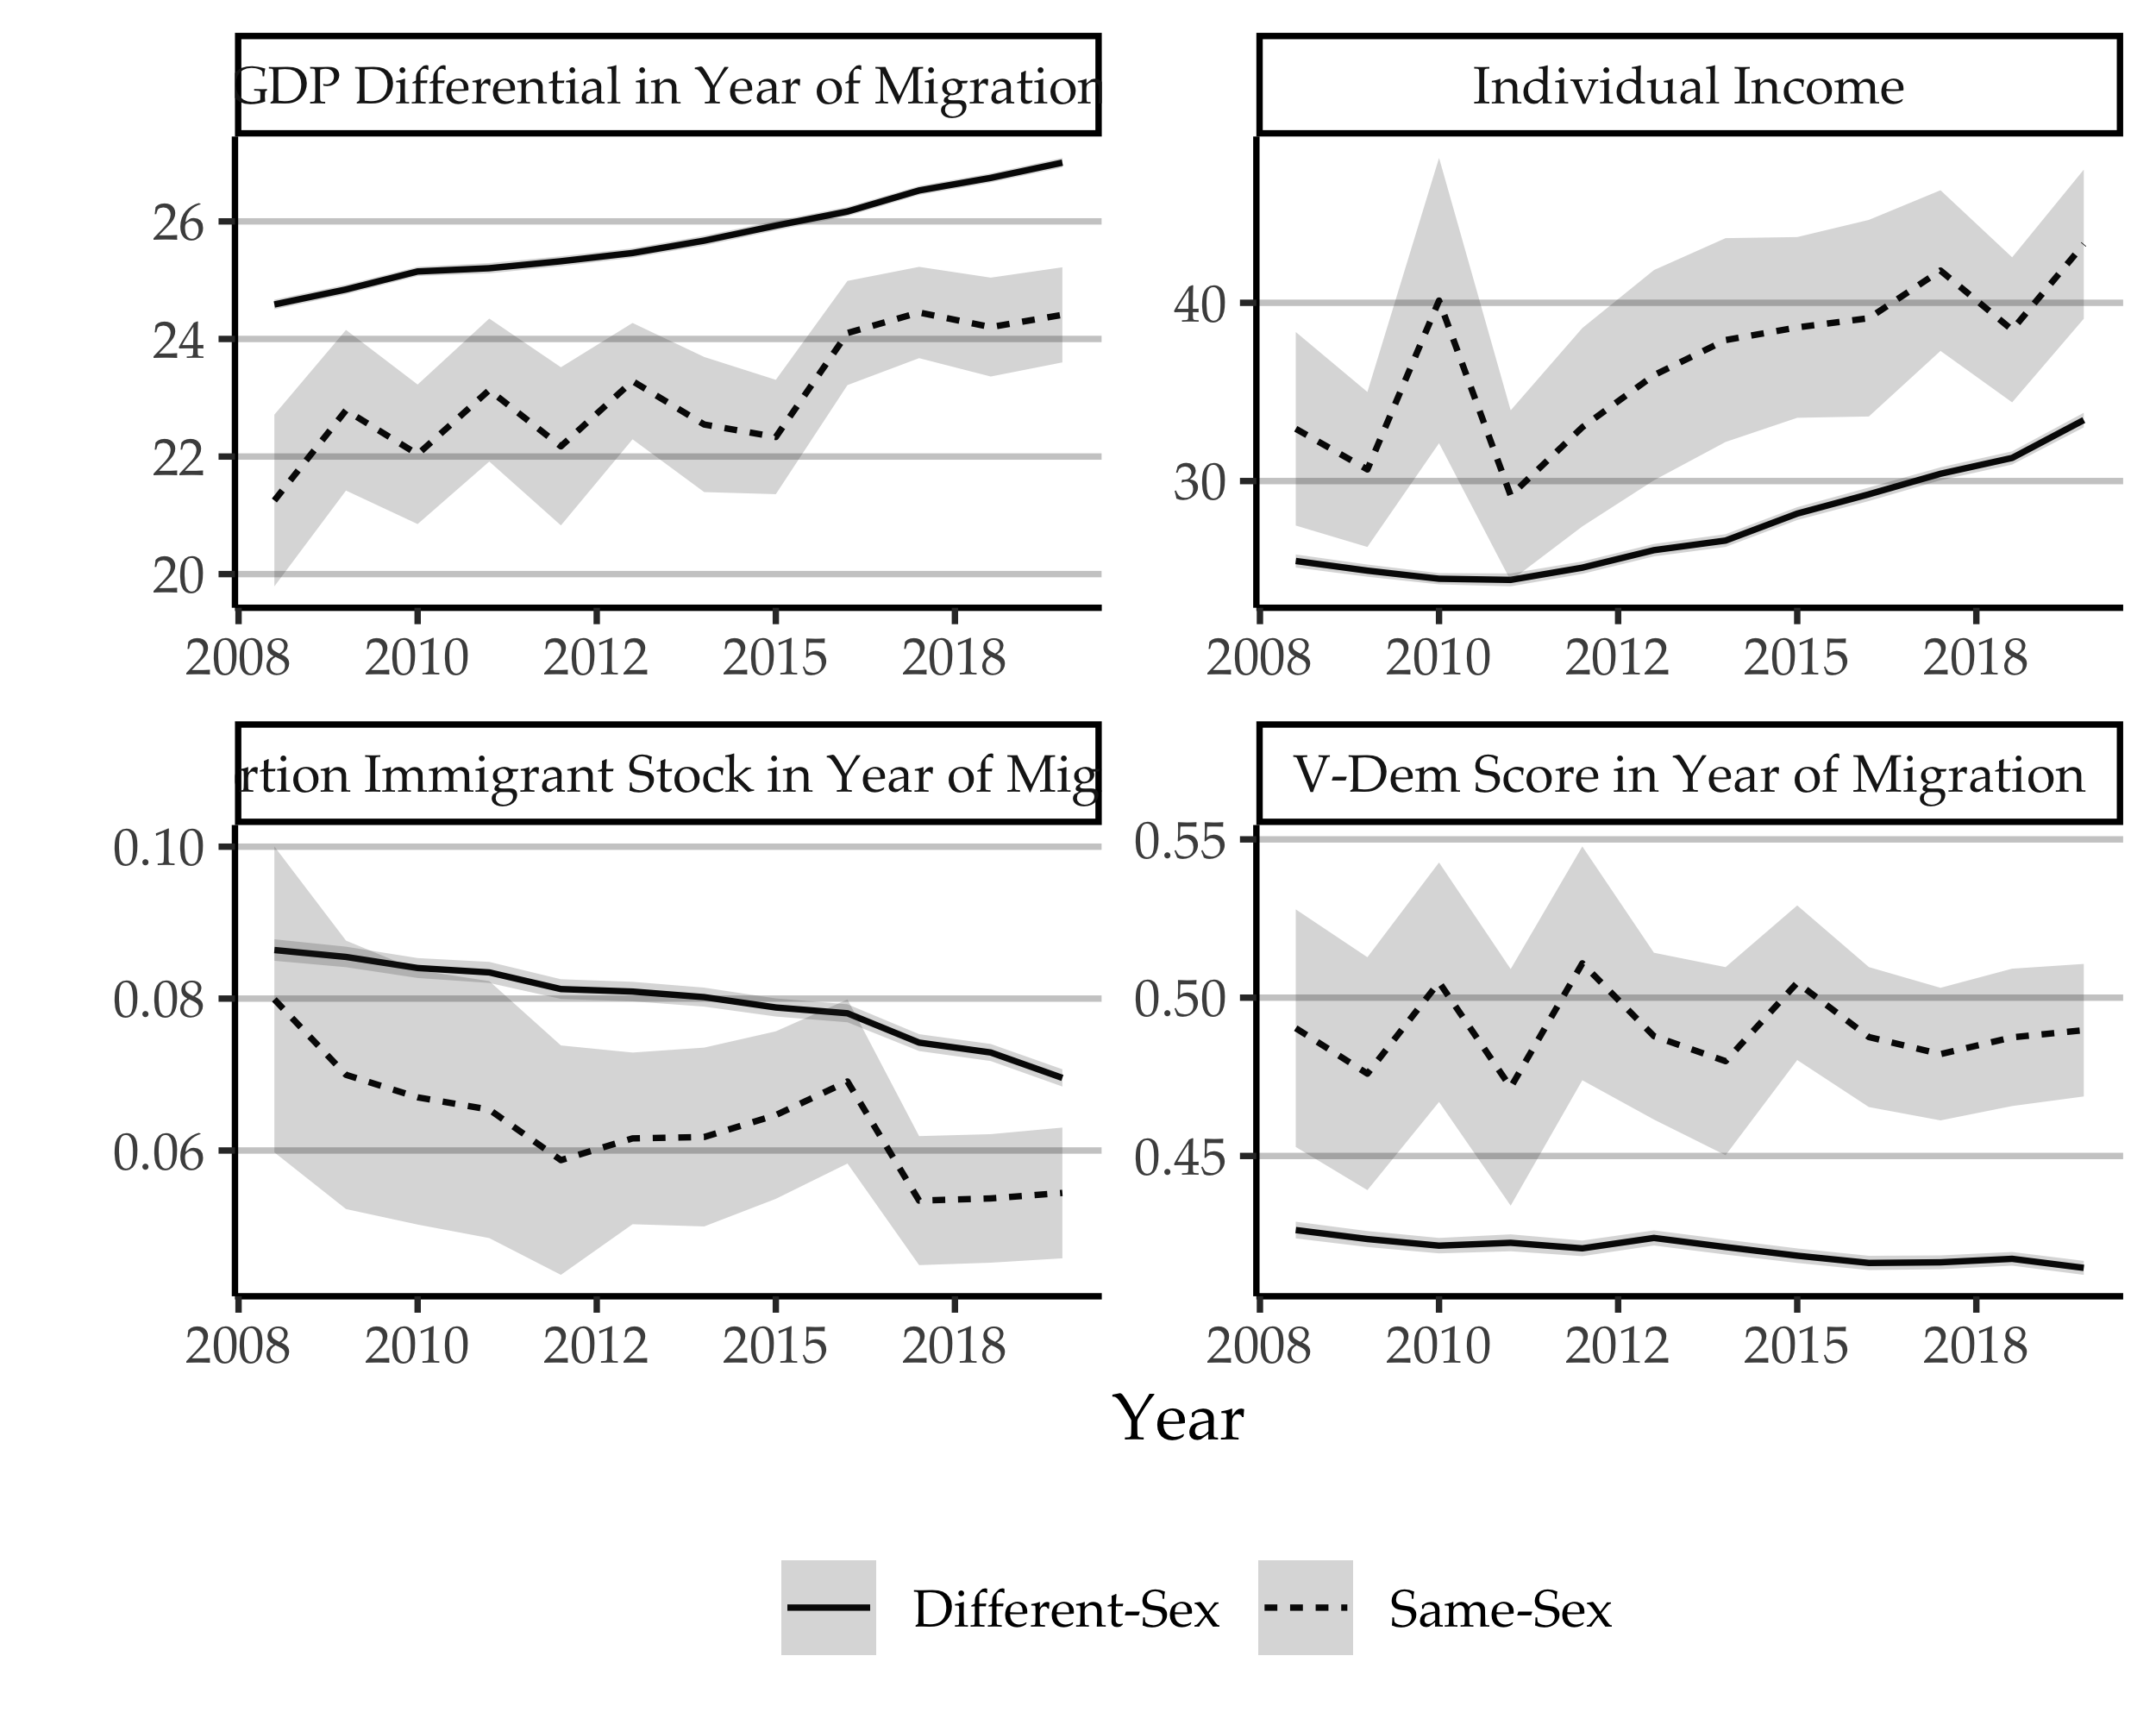
\includegraphics{ssimm_draft_files/figure-latex/desc-1.pdf}
\caption{\label{fig:desc}Descriptive statistics for immigrants in couples 2008-2019, with survey weights and 95\% confidence intervals. All currency in 1000s of 1999 dollars.}
\end{figure}

How do same- and different-sex immigrant couples differ in their individual attributes? Do variables of typical ``gravity models'' for migration differ between the groups? Figure \ref{fig:desc} compares immigrants in same- and different-sex couples on four variables. First, macroeconomic theory predicts that difference in wages across countries is one of the most important motivations for migration. The first panel in Figure \ref{fig:desc} shows that the wage differential is indeed positive for both groups of immigrants, it is significantly more positive for immigrants in different-sex couples. Statistics for the unemployment rate differential (now shown) indicate similar trends: LGB immigrants come from countries with lower unemployment rates. These findings indicate that macroeconomic considerations may be less important to migration of LGB immigrants. The second panel corroborates this finding on the individual level: not only do immigrants in same-sex couples come from countries with higher per capita GDP, but they individually tend to earn more than immigrants in different-sex couples. Additional analyses (not shown) demonstrate that immigrants in same-sex couples also tend to work in professions with higher occupational prestige scores and have somewhat higher education, indicating that they may come from more privileged social origins than their heterosexual counterparts.

Panel three of Figure \ref{fig:desc} compares democratization level of country of origin at time of migration for immigrants in our study. We see that this democratization level tends to be higher for immigrants in same-sex couples, indicating that political context may play a more important role in their migration. Finally, the fourth panel of Figure \ref{fig:desc} looks at per capita income of U.S. state of residence for the two groups. Although same-sex couples tend to live in states with higher income, the difference is small.

Although we see significant differences between same- and different-sex couples on a number of important migration variables, none shows the sudden jump in recent years reflected in Figure \ref{fig:total-pop}. Turning to LGBT policy may better explain this surge. Figure \ref{fig:policy-desc} charts the average country-of-origin and U.S.-state policy score for the immigrants in our sample over time, comparing means for immigrants in same- and different-sex couples. The left panel shows that country-of-origin index at time of migration is generally higher for immigrants in same-sex couples, and since 2013 it has rapidly increased. Immigrants in same-sex couples tend to come from more progressive countries, and this trend tracks closely with the overall population of this group. The right panel indicates less of a difference in U.S. state policies, although states where immigrants in same-sex couples live tend to score somewhat higher.

\begin{figure}
\centering
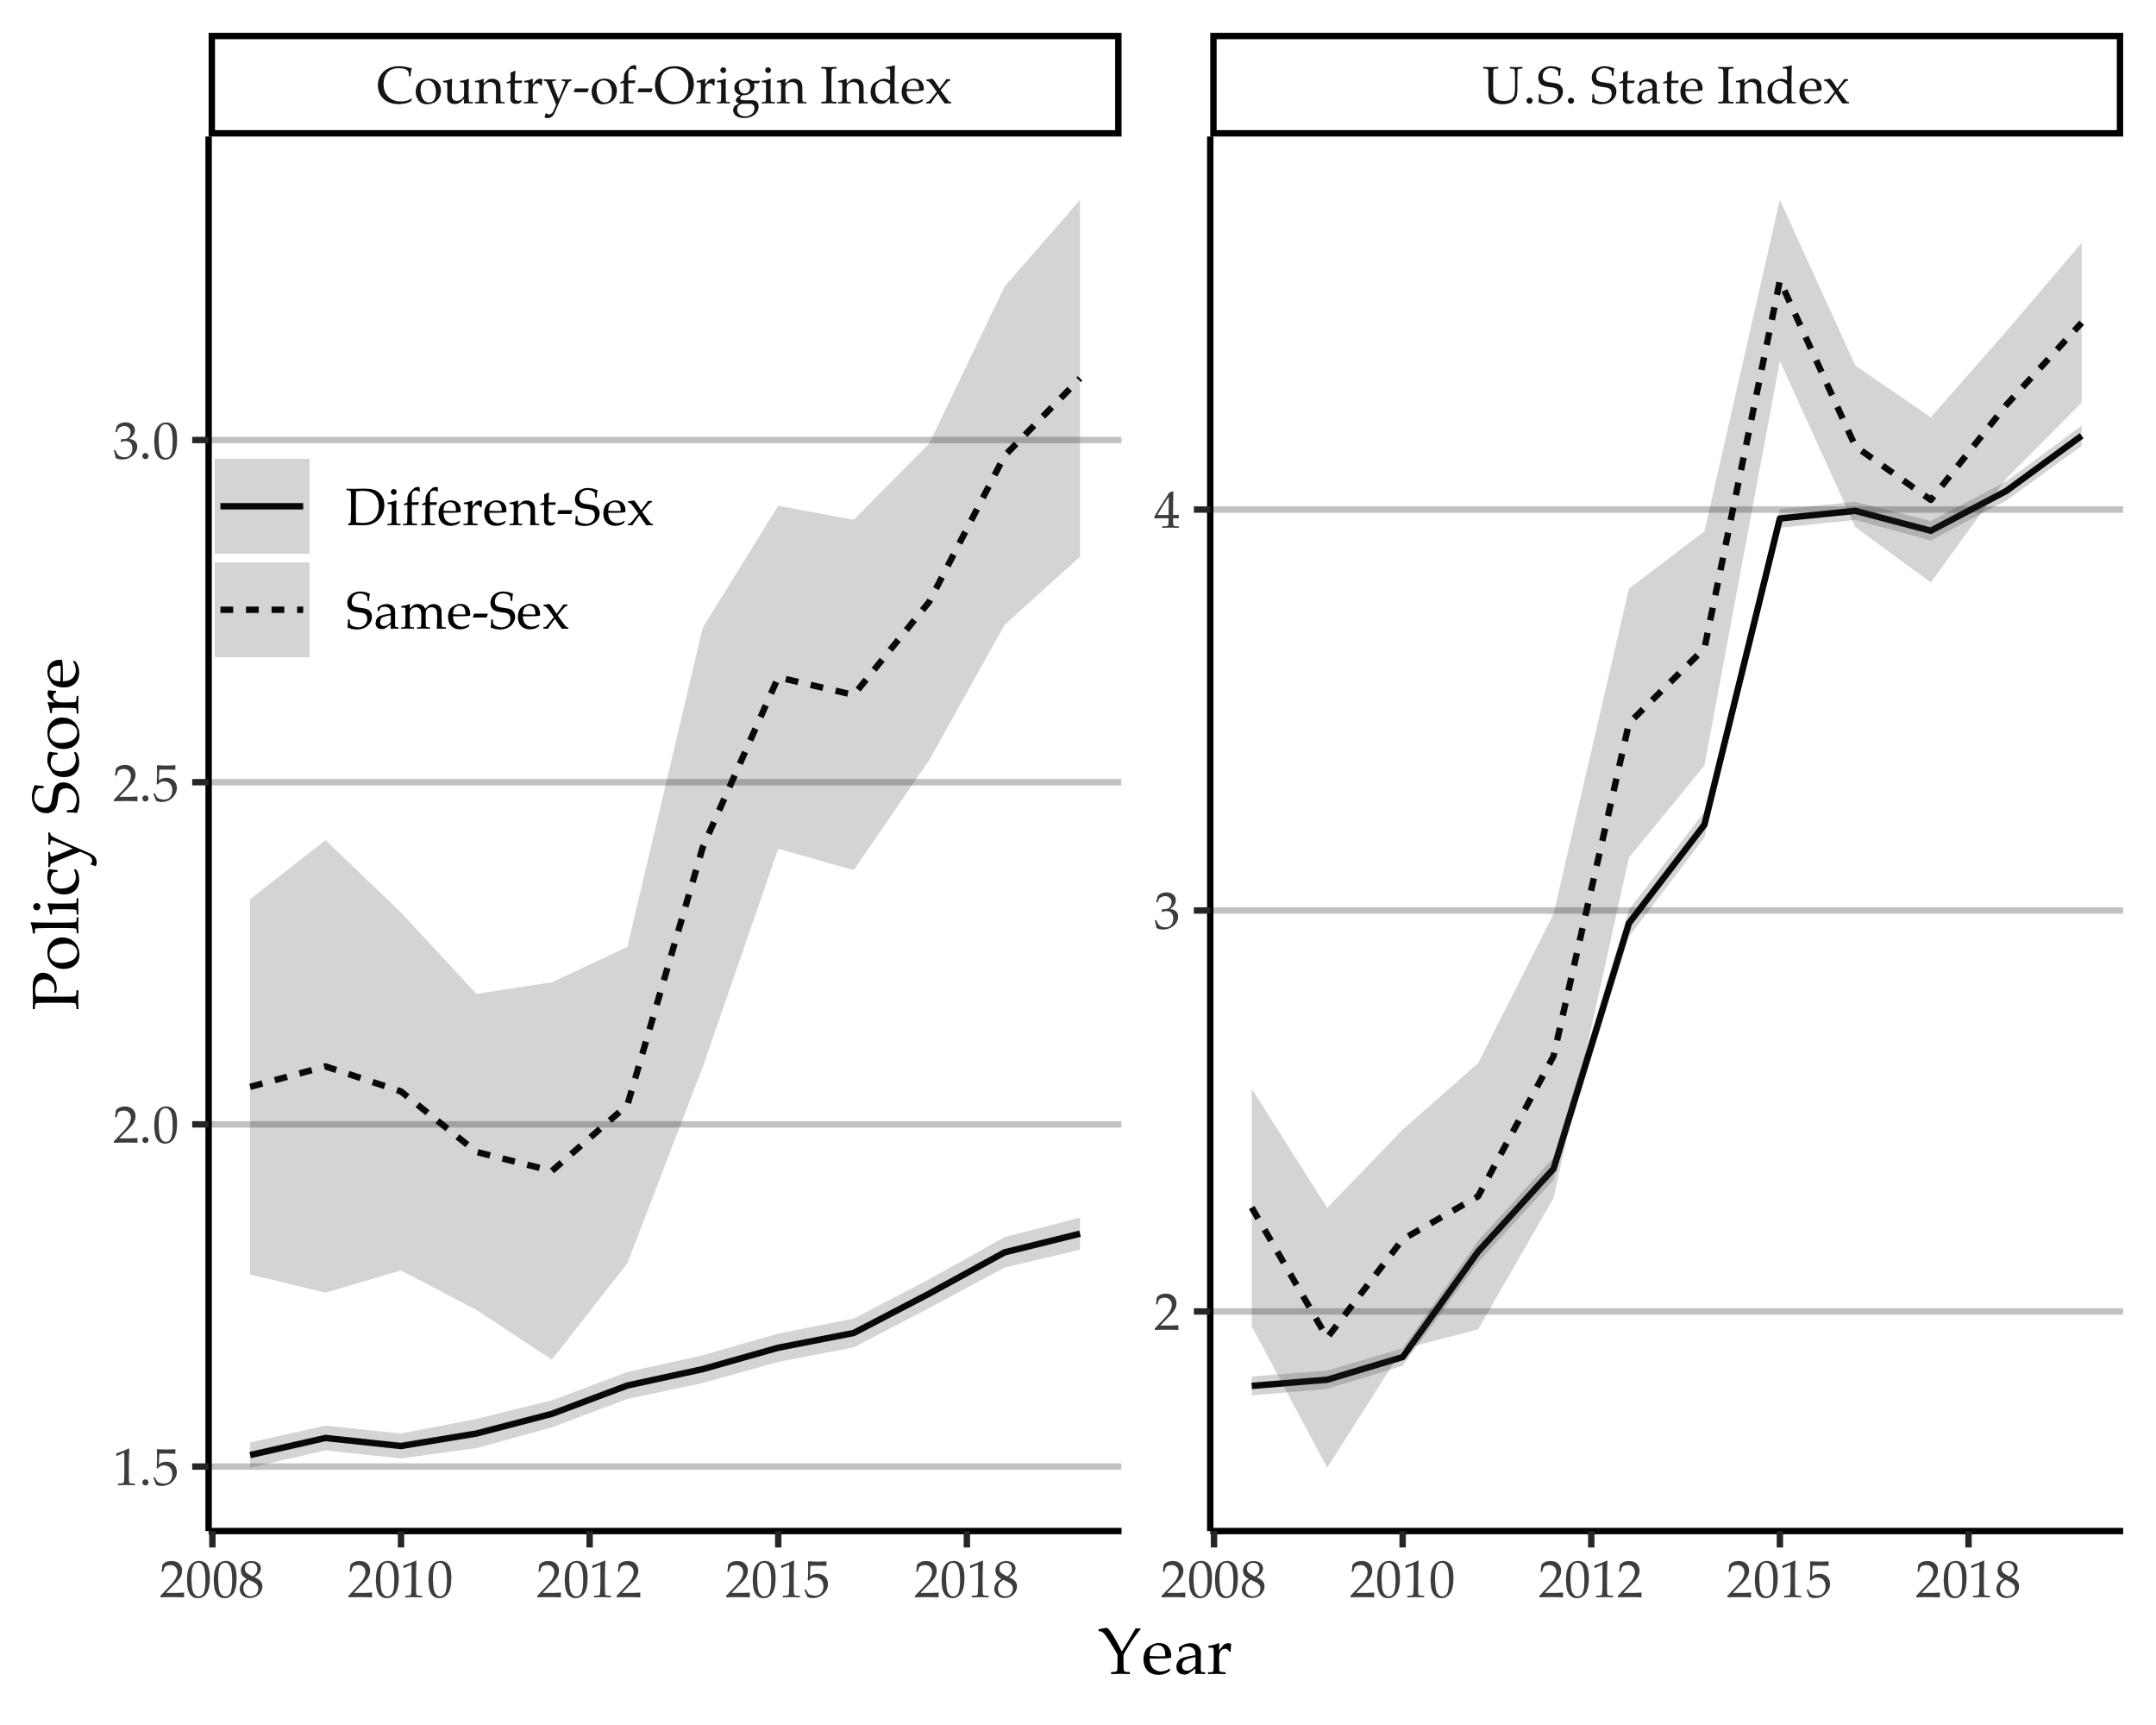
\includegraphics{ssimm_draft_files/figure-latex/policy-desc-1.pdf}
\caption{\label{fig:policy-desc}Mean country-of-origin and U.S. state policy index score for immigrants in same- and different-sex couples, 2008-2019, with 95\% confidence intervals.}
\end{figure}

\begin{table}

\caption{\label{tab:country-tab}Sending countries ranked bby proportion immigrant couples with same-sex partners}
\centering
\begin{tabular}[t]{lllr}
\toprule
Rank & Country of origin & Proportion same-sex & Mean policy score\\
\midrule
1 & Australia & 2.53 \% & 4.07\\
2 & Mongolia & 2.37 \% & 2.25\\
3 & Belgium & 2.2 \% & 4.97\\
4 & Singapore & 2.12 \% & -0.20\\
5 & Netherlands & 2.06 \% & 7.15\\
6 & Malaysia & 2.05 \% & -0.89\\
7 & France & 2.04 \% & 6.06\\
8 & New Zealand & 2.03 \% & 5.43\\
9 & Zimbabwe & 2.01 \% & -0.95\\
10 & Spain & 1.99 \% & 5.57\\
\bottomrule
\multicolumn{4}{l}{\rule{0pt}{1em}\textit{Source:} American Community Survey 2008-2019. Authors' calculations.}\\
\end{tabular}
\end{table}

\begin{table}

\caption{\label{tab:state-tab}States ranked by proportion immigrant couples with same-sex partners}
\centering
\begin{tabular}[t]{lllr}
\toprule
Rank & State & Proportion same-sex & Mean policy score\\
\midrule
1 & Vermont & 2.09 \% & 5.17\\
2 & Maine & 1.63 \% & 4.79\\
3 & Montana & 1.47 \% & 0.80\\
4 & Missouri & 1.18 \% & 1.91\\
5 & Massachusetts & 1.12 \% & 4.77\\
6 & New York & 1.10 \% & 4.85\\
7 & Florida & 1.01 \% & 0.91\\
8 & Mississippi & 1.00 \% & -0.49\\
9 & Minnesota & 0.96 \% & 4.63\\
10 & New Hampshire & 0.95 \% & 4.33\\
\bottomrule
\multicolumn{4}{l}{\rule{0pt}{1em}\textit{Source:} American Community Survey 2008-2019. Authors' calculations.}\\
\end{tabular}
\end{table}

Table \ref{tab:country-tab} ranks the proportion of U.S. immigrants in same-sex couples based on country of origin, averaging over the 11 years of survey data. The top sending countries mostly hold more progressive policies, but Singapore, Malaysia, and Zimbabwe maintain generally repressive policies at the year of departure of the immigrants in our sample. Table \ref{tab:state-tab} similarly ranks U.S. state by the proportion of immigrants in same-sex couples, averaging over the period of interest. Although states with progressive policies make the top of the list, Mississippi is somewhat repressive, and Montana, Missouri, and Florida hold more neutral policies.

\hypertarget{models}{%
\subsection{Models}\label{models}}

\begin{table}[!htbp] \centering 
  \caption{Percent of immigrants in same-sex couples by year of immigration and country of origin. Standard errors shown in parentheses, which are country-clustered for models 1, 2, and 3. Country controls include population-weighted distance, contiguous border, common official language, common ethnic language, colonial relationship, wage differential, unemployment differential, and Polity 5 measure of democratization.} 
  \label{tab:country-props} 
\begin{tabular}{@{\extracolsep{5pt}}lcccc} 
\\[-1.8ex]\hline 
\hline \\[-1.8ex] 
 & \multicolumn{4}{c}{\textit{Dependent variable:}} \\ 
\cline{2-5} 
\\[-1.8ex] & \multicolumn{4}{c}{prop\_same\_sex} \\ 
\\[-1.8ex] & (1) & (2) & (3) & (4)\\ 
\hline \\[-1.8ex] 
 polity5 &  & 0.016$^{***}$ & $-$0.004 & 0.012$^{*}$ \\ 
  &  & (0.004) & (0.007) & (0.005) \\ 
  & & & & \\ 
 origin\_score & 0.079$^{***}$ & 0.054$^{***}$ & 0.039$^{**}$ & 0.057$^{***}$ \\ 
  & (0.008) & (0.009) & (0.015) & (0.011) \\ 
  & & & & \\ 
\hline \\[-1.8ex] 
Country controls? & no & yes & yes & yes \\ 
Country FEs? & no & no & yes & no \\ 
Country REs? & no & no & no & yes \\ 
Observations & 3,222 & 3,222 & 3,222 & 3,222 \\ 
\hline 
\hline \\[-1.8ex] 
\multicolumn{5}{l}{Note: †p<0.1; *p<0.05; **p<0.01; ***p<0.001} \\ 
\multicolumn{5}{l}{Source: American Community Survey 2008-2019} \\ 
\end{tabular} 
\end{table}

Our first set of models predicts the percent of immigrants in same-sex couples by country of origin and year of immigration (Table \ref{tab:country-props}). Model 1 regresses this proportion on only our variable of interest: LGBT policy score in country of origin. We see that countries with more progressive LGBT policy tend to send more immigrants to the U.S. who end up in same-sex couples. The average proportion of immigrants in same-sex couples is only \texttt{r}mean(acs\_prop\_yrimmig\_policy\$prop\_same\_sex, na.rm = T)` percent, so an increase of 0.079 per point increase in LGBT policy score represents a substantive effect.

The other models in Table \ref{tab:country-props} assess the robustness of this finding. Model 2 includes typical controls from gravity models of immigration (e.g. \protect\hyperlink{ref-fitzgerald_2014}{Fitzgerald, Leblang, and Teets 2014}) along with a measure of democratization. The coefficient for country-of-origin score reduces slightly but remains highly significant. Notably, it is estimated to be more than three times the effect size of democratization score; the LGBT policy environment matters much more than the overall progressiveness of government policy. Models 3 and 4 include country-of-origin fixed and random effects, respectively. Although in the fixed effects model coefficient for origin score is reduced by half compared to Model 1, it remains statistically significant. The corresponding coefficient random effects model remains large and significant.

\begin{table}[!htbp] \centering 
  \caption{Percent same-sex in by country of origin, U.S. state, and survey year. Country-clustered standard errors are shown in parentheses. State controls include unemployment rate and per-capita income. Country controls include population-weighted distance, contiguous border, common official language, common ethnic language, colonial relationship, wage differential, unemployment differential, and Polity 5 measure of democratization.} 
  \label{tab:state-props} 
\begin{tabular}{@{\extracolsep{5pt}}lccc} 
\\[-1.8ex]\hline 
\hline \\[-1.8ex] 
 & \multicolumn{3}{c}{\textit{Dependent variable:}} \\ 
\cline{2-4} 
\\[-1.8ex] & \multicolumn{3}{c}{same\_prop} \\ 
\\[-1.8ex] & (1) & (2) & (3)\\ 
\hline \\[-1.8ex] 
 origin\_score & 0.050$^{***}$ & 0.048$^{***}$ & 0.130$^{***}$ \\ 
  & (0.011) & (0.011) & (0.040) \\ 
  & & & \\ 
 state\_policy & 0.041$^{*}$ & 0.019 & 0.035 \\ 
  & (0.018) & (0.034) & (0.034) \\ 
  & & & \\ 
\hline \\[-1.8ex] 
State controls and FEs? & no & yes & yes \\ 
Country controls and FEs? & no & no & yes \\ 
Observations & 39,458 & 39,458 & 39,458 \\ 
\hline 
\hline \\[-1.8ex] 
\multicolumn{4}{l}{Note: †p<0.1; *p<0.05; **p<0.01; ***p<0.001} \\ 
\multicolumn{4}{l}{Source: American Community Survey 2008-2019} \\ 
\end{tabular} 
\end{table}

Table \ref{tab:state-props} presents models of U.S. state-level proportion of immigrants in same-sex couples, from a given country of origin in a given survey year. Model 1 contains only two predictors: U.S. state policy score in the survey year and country-of-origin policy score at the mean year of immigration. Although more LGBT-friendly policies in both locations are associated with higher numbers of immigrants in same-sex couples, country-of-origin LGBT policy is a stronger predictor than U.S. state policy, even considering the somewhat different scale of these variables. A one-standard deviation increase origin score is associated with a 0.098 percentage-point increase of immigrants in same-sex couples, whereas the corresponding state policy effect is 0.1 percentage points.

Model 2 adds state-level controls and fixed effects. Immigrants in same-sex couples may be attracted to progressive states for their economic rather than political benefits. Indeed, in this model, the coefficient for state policy is reduced and rendered insignificant. Model 3 adds country-of-origin controls and fixed effects. The state policy effect remains imprecisely estimated, but country-of-origin policy has increased in strength. More progressive sending countries are more represented among same-sex couples, while U.S. state policy appears to have little influence on their settlement patterns, at least in the aggregate.

\begin{table}[!htbp] \centering 
  \caption{Individual ordered logit analysis of three-category state policy score. Country-clustered standard errors are shown in parentheses. Individual controls include sex, age, education, number of children, log(income), indicator for no income, and year of immigration, which are all interacted with the indicator for same-sex couple.} 
  \label{tab:ord} 
\begin{tabular}{@{\extracolsep{5pt}}lccc} 
\\[-1.8ex]\hline 
\hline \\[-1.8ex] 
 & \multicolumn{3}{c}{\textit{Dependent variable:}} \\ 
\cline{2-4} 
\\[-1.8ex] & \multicolumn{3}{c}{state\_policy\_binned} \\ 
\\[-1.8ex] & (1) & (2) & (3)\\ 
\hline \\[-1.8ex] 
 same\_sex & $-$0.046$^{*}$ & $-$0.044$^{†}$ & $-$5.500$^{***}$ \\ 
  & (0.020) & (0.027) & (0.0003) \\ 
  & & & \\ 
 origin\_score &  & 0.001 & 0.002 \\ 
  &  & (0.003) & (0.003) \\ 
  & & & \\ 
 same\_sexTRUE:origin\_score &  & $-$0.001 & $-$0.005 \\ 
  &  & (0.008) & (0.008) \\ 
  & & & \\ 
\hline \\[-1.8ex] 
Survey year FEs? & yes & yes & yes \\ 
Individual controls? & no & no & yes \\ 
Observations & 111,706 & 111,706 & 111,706 \\ 
\hline 
\hline \\[-1.8ex] 
\multicolumn{4}{l}{Note: †p<0.1; *p<0.05; **p<0.01; ***p<0.001} \\ 
\multicolumn{4}{l}{Source: American Community Survey 2008-2019} \\ 
\end{tabular} 
\end{table}

Our final set of models turn to the individual. Conditional on migrating to the U.S., do immigrants in same-sex couples choose to live in more progressive states than their heterosexual counterparts? Table \ref{tab:ord} presents ordered logit models predicting whether an individual partnered immigrant lives in a U.S. state with repressive, neutral, or progressive LGBT policies, pooling data across survey years. Model 1 includes only one regressor: an indicator for whether the immigrant is in a same-sex couple. The positive coefficient indicates that immigrants in same-sex couples indeed tend to live in states with more LGBT-friendly policies. The predicted probability for an immigrant in a different-sex couple to live in a state with progressive LGBT policies is 0.62, whereas the corresponding probability for those in same-sex couples is 0.62. At the repressive end of the policy spectrum, the predicted probabilities are 0.22 and 0.22 for different- and same-sex couples, respectively.

How does country-of-origin context mediate this results? Model 2 adds sending-country LGBT policy score at the time of immigration to the regression, interacting it with the same-sex indicator. The coefficient for the same-sex indicator remains positive and significant, but we see opposite effects of the origin-score coefficient for immigrants in different- and same-sex couples. For different-sex couples, hailing from a more progressive country is associated with living in a more repressive U.S. state. For same-sex couples, the result is in the opposite direction: those from progressive countries tend to live in more progressive U.S. states.

Model 3 controls for possible individual confounders, interacting them with the same-sex indicator. If immigrants in same-sex couples also tend to have more education, higher income, different family structures, or less years of age, they may be choosing more progressive states due to other policies or economic conditions. As shown in Table \ref{tab:ord}, the effects from Model 2 remain strong and in the same directions.

\begin{figure}
\centering
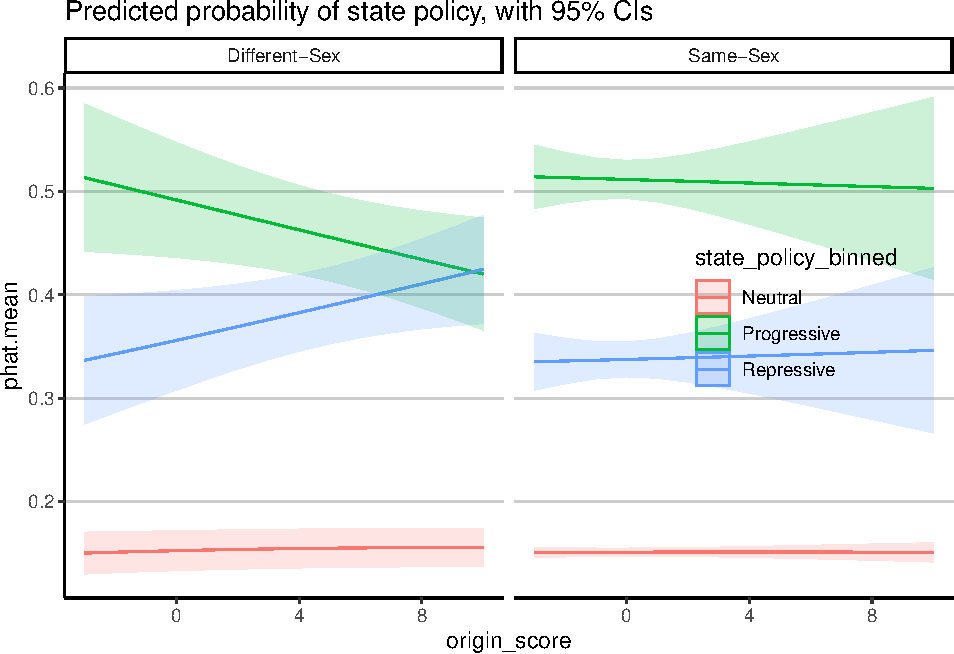
\includegraphics{ssimm_draft_files/figure-latex/sim-1.pdf}
\caption{\label{fig:sim}Predicted probabilities of U.S. state LGBT policy progressiveness for individual immigrants in different- and same-sex couples, based on policy score of sending country, with 95\% confidence intervals.}
\end{figure}

To help interpret these results, Figure \ref{fig:sim} contains predicted probabilities of residing in progressive, neutral, or repressive U.S. states. Each panel predicts these probabilities for a typical immigrant in the dataset, based on means for continuous and modes for categorical variables while varying sending-country policy score. The only difference between the two panels is the value for the same-sex indicator.

The figure shows opposite trends for same- and different-sex couples. Overall, immigrants tend to live in more progressive states, but the moderating effect of origin score is quite different for the two groups. The panel for same-sex couples shows that these immigrants tend to live in U.S. states with similar LGBT policy contexts to those of their countries of origin. Immigrants in same-sex couples from more repressive countries are less likely to live in more progressive U.S. states, but as the origin-country score increases, so does the probability of living in a progressive state For immigrants in different-sex couples, on the other hand, increasingly progressive country-of-origin policies are associated with a \emph{lower} probability of residing in a progressive U.S. state, accompanied by a \emph{higher} probability of living in a repressive U.S. state. At the high end of the origin-score policy range, the difference in predicted probabilities is significant: typical immigrants in same-sex couples are 0.82 percentage points more likely to live in progressive states and -0.82 percentage points less likely to live in repressive states.

\hypertarget{discussion}{%
\section{Discussion}\label{discussion}}

In 2000, there were 35,820 self-reported same-sex immigrant couples. By 2019, this number tripled to over 108,000 (\protect\hyperlink{ref-u.s.censusbureau_2020}{U.S. Census Bureau 2020}). Despite this expansive growth of same-sex immigrant couples in the U.S., there is little demographic research understanding the characteristics of these couples or the factors influencing their migratory patterns. Consequently, we know little about who these migrants are, why they are choosing to leave their home countries, or where they are choosing to locate once in the U.S. Answering these questions is important, not just because this represents an increasing number of people, but because it has the potential to reshape our conceptualization of who immigrants are and their motivations for moving.

The rising number of same-sex immigrant couples has coincided with a dramatic change in policy environments governing LGBT communities -- both within the U.S. and abroad. Indeed, it is precisely because of this changing policy environment, namely around the 2013 DOMA Supreme Court case, that same-sex couples now have a legal pathway into the U.S. that does not rely on asylum claims. Therefore, although there are numerous perspectives to take in understanding the migratory patterns of these couples, this project specifically investigates how changing LGBT policies at both country of origin and residing U.S. state pattern these migratory pathways. Engaging in such a question adds to emerging scholarship trying to understand how dramatic policy changes are influencing the health, well-being, and lifestyles of LGBT people while also recognizing that these policies differentially impact people within this broad umbrella based on different social positions (xx). Moreover, it helps to address an important gap within migration studies that too often discount the role of the state and the salience of sexuality in conditioning migratory patterns (\protect\hyperlink{ref-carrillo_2018}{Carrillo 2018}; \protect\hyperlink{ref-fitzgerald_2014}{Fitzgerald, Leblang, and Teets 2014}).

To answer this question, we take advantage of an underutilized data source: self-reports of same-sex immigrant couples in the American Community Survey from 2008-2019. Despite this resource being one of the few national surveys to capture same-sex couples, let alone immigrant couples, these data are virtually untapped. Few studies take advantage of this data source, and the ones that do largely focus on residential segregation (\protect\hyperlink{ref-poston_2017}{Poston et al. 2017}). Therefore, these data allow for us to make one of the first large-\(N\) investigations of same-sex immigrant couples within the U.S. and to make an important correction to this area of scholarship.

Through these data, we make a number of interesting findings worth detailing. First, existing scholarship on same-sex immigrant couples, and queer migration more broadly, largely focuses on the asylum and refugee processes. This is because this was one of the only mechanisms to get into the U.S. (\protect\hyperlink{ref-humanrightswatch_2006}{Watch 2006}); xx). Consequently, this over-representation distorts our understanding of who same-sex immigrant couples are, the types of environments they are leaving from, and their motivations to seek entry into the U.S. Indeed, when comparing the demographics of same-sex immigrant couples to different-sex immigrant couples, we find same-sex couples generally have higher incomes and occupational prestige and are somewhat more educated. Understanding this profile alone is an important insight, as it reveals that these communities are of privileged social standing. This is not necessarily surprising, however, considering that migrating is often an expensive and intensive process.

Understanding who these migrants are, how do LGBT policies in their countries of origin influence their desires to come to the U.S.? Despite existing scholarship portraying a story of LGB couples fleeing repression, as necessary for refugee claims, LGB couples are leaving countries with more progressive policy environments. As results in Table \ref{tab:country-props} and trendlines in Figure \ref{fig:policy-desc} reveal, couples are coming from more open environments. This is true even after accounting for more traditional gravity model variables that primarily focus on economic costs and benefits to migration. Though more research is needed, these results, in conjunction with the fact that these same-sex couples have higher incomes and greater occupational prestige, describe a situation in which perhaps it is the supportive policy environment, such as employment protections, access to the material benefits of marriage, and so forth, that enable same-sex couples to achieve greater social standing and the resources necessary to migrate. Or, instead of the immediate benefits of the policy itself, these supportive environments may simply encourage LGB people to feel comfortable to openly identify as being in a relationship.

One unexpected finding is that as different-sex couples come from more supportive countries, this is associated with residing in states with increasingly less LGBT-friendly policies. These patterns in Figure \ref{fig:sim} are peculiar because we suspected state LGBT policies to have no association with how different-sex couples are making decisions as to where to reside. This is not the case. One immediate question this raises is if this is a case of ``straight flight?'' White flight is a well-research process in which white people leave diversifying communities. After straight couples experience liberalized conditions for gay couples, do they intentionally seek to leave such conditions by moving to states that are less supportive? More research is needed to understand this pattern.

While gender has been recently recognized as an integral part of the migration process (\protect\hyperlink{ref-lutz_2010}{Lutz 2010}; \protect\hyperlink{ref-hondagneu-sotelo_2012}{Hondagneu-Sotelo 2012}), sexuality has thus far received relatively scant attention. As Carrillo (\protect\hyperlink{ref-carrillo_2018}{2018}) demonstrates, however, sexuality is a salient factor determining immigration decisions. We show that differences between immigrants in same-sex couples and those in different-sex couples cannot be explained solely using classic theories of migration; consequently, by not making sexuality an integral part of the research question, this limits our understanding of the full immigration process.

\hypertarget{references}{%
\section{References}\label{references}}

\setlength{\parindent}{-0.2in}
\setlength{\leftskip}{0.2in}
\setlength{\parskip}{8pt}

\noindent

\hypertarget{refs}{}
\begin{CSLReferences}{1}{0}
\leavevmode\hypertarget{ref-adur_2018}{}%
Adur, Shweta Majumdar. 2018. {``In Pursuit of Love: {`{Safe} Passages,'} Migration and Queer {South} {Asians} in the {US}.''} \emph{Current Sociology} 66 (2): 320--34.

\leavevmode\hypertarget{ref-anderson_2011}{}%
Anderson, James E. 2011. {``The {Gravity} {Model}.''} \emph{Annual Review of Economics} 3 (1): 133--60. \url{https://doi.org/10.1146/annurev-economics-111809-125114}.

\leavevmode\hypertarget{ref-ayoub_2016}{}%
Ayoub, Phillip. 2016. \emph{When {States} {Come} {Out}}. Cambridge University Press.

\leavevmode\hypertarget{ref-ayoub_2017}{}%
Ayoub, Phillip, and Jeremiah Garretson. 2017. {``Getting the Message Out: {Media} Context and Global Changes in Attitudes Toward Homosexuality.''} \emph{Comparative Political Studies} 50 (8): 1055--85.

\leavevmode\hypertarget{ref-beaudin_2017}{}%
Beaudin, Laura. 2017. {``Marriage Equality and Interstate Migration.''} \emph{Applied Economics} 49 (30): 2956--73. \url{https://doi.org/10.1080/00036846.2016.1251565}.

\leavevmode\hypertarget{ref-boertien_2019}{}%
Boertien, Diederik, and Daniele Vignoli. 2019. {``Legalizing Same-Sex Marriage Matters for the Subjective Well-Being of Individuals in Same-Sex Unions.''} \emph{Demography} 56 (6): 2109--21.

\leavevmode\hypertarget{ref-canaday_2009}{}%
Canaday, Margot. 2009. \emph{The Straight State: Sexuality and Citizenship in Twentieth-Century {America}}. Politics and Society in Twentieth-Century {America}. Princeton, N.J: Princeton University Press.

\leavevmode\hypertarget{ref-cantu_2009}{}%
Cantú, Lionel. 2009. \emph{The {Sexuality} of {Migration}: {Border} {Crossings} and {Mexican} {Immigrant} {Men}}. Edited by Nancy A. Naples and Salvador Vidal-Ortiz. New York: NYU Press.

\leavevmode\hypertarget{ref-carpenter_2020}{}%
Carpenter, Christopher S. 2020. {``The {Direct} {Effects} of {Legal} {Same}-{Sex} {Marriage} in the {United} {States}: {Evidence} {From} {Massachusetts}.''} \emph{Demography} 57 (5): 1787--1808.

\leavevmode\hypertarget{ref-carrillo_2018}{}%
Carrillo, Héctor. 2018. \emph{Pathways of {Desire}: {The} {Sexual} {Migration} of {Mexican} {Gay} {Men}}. University of Chicago Press.

\leavevmode\hypertarget{ref-corey-boulet_2019}{}%
Corey-Boulet, Robbie. 2019. \emph{Love {Falls} on {Us}: A Story of {American} Ideas and {African} {LGBT} Lives}. Zed Books Ltd.

\leavevmode\hypertarget{ref-epstein_2014}{}%
Epstein, Steven, and Héctor Carrillo. 2014. {``Immigrant Sexual Citizenship: Intersectional Templates Among {Mexican} Gay Immigrants to the {USA}.''} \emph{Citizenship Studies} 18 (3-4): 259--76. \url{https://doi.org/10.1080/13621025.2014.905266}.

\leavevmode\hypertarget{ref-feenstra_2015}{}%
Feenstra, Robert C., Robert Inklaar, and Marcel P. Timmer. 2015. {``The {Next} {Generation} of the {Penn} {World} {Table}.''} \emph{American Economic Review} 105 (10): 3150--82. \url{https://doi.org/10.1257/aer.20130954}.

\leavevmode\hypertarget{ref-feliciano_2020}{}%
Feliciano, Cynthia. 2020. {``Immigrant {Selectivity} {Effects} on {Health}, {Labor} {Market}, and {Educational} {Outcomes}.''} \emph{Annual Review of Sociology} 46 (1): 315--34. \url{https://doi.org/10.1146/annurev-soc-121919-054639}.

\leavevmode\hypertarget{ref-fitzgerald_2014}{}%
Fitzgerald, Jennifer, David Leblang, and Jessica C. Teets. 2014. {``Defying the {Law} of {Gravity}: {The} {Political} {Economy} of {International} {Migration}.''} \emph{World Politics} 66 (3): 406--45. \url{https://doi.org/10.1017/S0043887114000112}.

\leavevmode\hypertarget{ref-giametta_2020}{}%
Giametta, Calogero. 2020. {``New Asylum Protection Categories and Elusive Filtering Devices: The Case of {`{Queer} Asylum'} in {France} and the {UK}.''} \emph{Journal of Ethnic and Migration Studies} 46 (1): 142--57.

\leavevmode\hypertarget{ref-gonzalez-lopez_2005}{}%
González-López, Gloria. 2005. \emph{Erotic {Journeys}}. University of California Press.

\leavevmode\hypertarget{ref-hatton_2005a}{}%
Hatton, Timothy J., and Jeffrey G. Williamson. 2005. \emph{Global {Migration} and the {World} {Economy}: {Two} {Centuries} of {Policy} and {Performance}}. The MIT Press. \url{https://doi.org/10.7551/mitpress/3303.001.0001}.

\leavevmode\hypertarget{ref-hondagneu-sotelo_2012}{}%
Hondagneu-Sotelo, Pierrette. 2012. {``New Directions in Gender and Immigration Research.''} In \emph{Routledge {International} {Handbook} of {Migration} {Studies}}. Routledge. \url{https://doi.org/10.4324/9780203863299.ch15}.

\leavevmode\hypertarget{ref-kail_2015}{}%
Kail, Ben Lennox, Katie L. Acosta, and Eric Wright. 2015. {``State-Level Marriage Equality and the Health of Same-Sex Couples.''} \emph{American Journal of Public Health} 105 (6): 1101--5.

\leavevmode\hypertarget{ref-karemera_2000}{}%
Karemera, David, Victor Iwuagwu Oguledo, and Bobby Davis. 2000. {``A Gravity Model Analysis of International Migration to {North} {America}.''} \emph{Applied Economics} 32 (13): 1745--55. \url{https://doi.org/10.1080/000368400421093}.

\leavevmode\hypertarget{ref-karimi_2020}{}%
Karimi, Ayran. 2020. {``Refugees' {Transnational} {Practices}: {Gay} {Iranian} {Men} {Navigating} {Refugee} {Status} and {Cross}-Border {Ties} in {Canada}.''} \emph{Social Currents} 7 (1): 71--86.

\leavevmode\hypertarget{ref-lax_2009}{}%
Lax, Jeffrey R., and Justin H. Phillips. 2009. {``Gay Rights in the States: {Public} Opinion and Policy Responsiveness.''} \emph{American Political Science Review} 103 (3): 367--86.

\leavevmode\hypertarget{ref-levy_2017}{}%
Levy, Brian L., and Denise L. Levy. 2017. {``When {Love} {Meets} {Hate}: {The} {Relationship} {Between} {State} {Policies} on {Gay} and {Lesbian} {Rights} and {Hate} {Crime} {Incidence}.''} \emph{Social Science Research} 61: 142--59.

\leavevmode\hypertarget{ref-luibheid_2008}{}%
Luibhéid, E. 2008. {``Queer/{Migration}: {An} {Unruly} {Body} of {Scholarship}.''} \emph{GLQ: A Journal of Lesbian and Gay Studies} 14 (2-3): 169--90. \url{https://doi.org/10.1215/10642684-2007-029}.

\leavevmode\hypertarget{ref-luibheid_2005}{}%
Luibhéid, Eithne, and Lionel Cantú. 2005. \emph{Queer {Migrations}: {Sexuality}, {U}.{S}. {Citizenship}, and {Border} {Crossings}}. U of Minnesota Press.

\leavevmode\hypertarget{ref-lutz_2010}{}%
Lutz, Helma. 2010. {``Gender in the {Migratory} {Process}.''} \emph{Journal of Ethnic and Migration Studies} 36 (10): 1647--63. \url{https://doi.org/10.1080/1369183X.2010.489373}.

\leavevmode\hypertarget{ref-mayer_2011}{}%
Mayer, Thierry, and Soledad Zignago. 2011. {``Notes on {CEPII}'s {Distances} {Measures}: {The} {GeoDist} {Database}.''} \emph{SSRN Electronic Journal}. \url{https://doi.org/10.2139/ssrn.1994531}.

\leavevmode\hypertarget{ref-mole_2018a}{}%
Mole, Richard. 2018. {``Sexualities and Queer Migration Research.''} \emph{Sexualities} 21 (8): 1268--70.

\leavevmode\hypertarget{ref-murray_2016}{}%
Murray, David A. B. 2016. \emph{Queering {Borders}: {Language}, {Sexuality}, and {Migration}}. John Benjamins Publishing Company.

\leavevmode\hypertarget{ref-palloni_2001}{}%
Palloni, Alberto, Douglas S. Massey, Miguel Ceballos, Kristin Espinosa, and Michael Spittel. 2001. {``Social {Capital} and {International} {Migration}: {A} {Test} {Using} {Information} on {Family} {Networks}.''} \emph{American Journal of Sociology} 106 (5): 1262--98. \url{https://doi.org/10.1086/320817}.

\leavevmode\hypertarget{ref-poot_2016}{}%
Poot, Jacques, Omoniyi Alimi, Michael P. Cameron, and David C. Maré. 2016. {``The {Gravity} {Model} of {Migration}: {The} {Successful} {Comeback} of an {Ageing} {Superstar} in {Regional} {Science}.''} SSRN Scholarly Paper ID 2864830. Rochester, NY: Social Science Research Network. \url{https://papers.ssrn.com/abstract=2864830}.

\leavevmode\hypertarget{ref-portes_1998}{}%
Portes, Alejandro. 1998. {``Social {Capital}: {Its} {Origins} and {Applications} in {Modern} {Sociology}.''} \emph{Annual Review of Sociology} 24 (1): 1--24. \url{https://doi.org/10.1146/annurev.soc.24.1.1}.

\leavevmode\hypertarget{ref-poston_2017}{}%
Poston, Dudley L. Jr, D'Lane R. Compton, Qian Xiong, and Emily A. Knox. 2017. {``The {Residential} {Segregation} of {Same}-{Sex} {Households} from {Different}-{Sex} {Households} in {Metropolitan} {USA}, Circa-2010.''} \emph{Population Review} 56 (2). \url{https://doi.org/10.1353/prv.2017.0005}.

\leavevmode\hypertarget{ref-soule_2004}{}%
Soule, Sarah. 2004. {``Going to the Chapel? {Same}-Sex Marriage Bans in the {United} {States}, 1973--2000.''} \emph{Social Problems} 51 (4): 453--77.

\leavevmode\hypertarget{ref-stella_2020}{}%
Stella, Francesca, and Anna Gawlewicz. 2020. {``Social Networks, Language and Identity Negotiations Among Queer Migrants in {Scotland}.''} \emph{Journal of Ethnic and Migration Studies}, 1--19.

\leavevmode\hypertarget{ref-todaro_1980}{}%
Todaro, Michael. 1980. {``Internal Migration in Developing Countries: A Survey.''} In \emph{Population and Economic Change in Developing Countries}, 361--402. Chicago: University of Chicago Press.

\leavevmode\hypertarget{ref-u.s.censusbureau_2013}{}%
U.S. Census Bureau. 2013. {``Frequently {Asked} {Questions} {About} {Same}-{Sex} {Couple} {Households}.''} U.S. Census Bureau Fertility; Family Statistics Branch.

\leavevmode\hypertarget{ref-u.s.censusbureau_2020}{}%
---------. 2020. {``2008-2019 {American} {Community} {Survey} {Public} {Use} {Microdata} {Samples}.''} \url{https://usa.ipums.org/usa/index.shtml}.

\leavevmode\hypertarget{ref-velasco_2018}{}%
Velasco, Kristopher. 2018. {``Human {Rights} {INGOs}, {LGBT} {INGOs}, and {LGBT} {Policy} {Diffusion}, 1991--2015.''} \emph{Social Forces} 97 (1): 377--404. \url{https://doi.org/10.1093/sf/soy030}.

\leavevmode\hypertarget{ref-velasco_2020}{}%
---------. 2020. {``A {Growing} {Queer} {Divide}: {The} {Divergence} Between {Transnational} {Advocacy} {Networks} and {Foreign} {Aid} in {Diffusing} {LGBT} {Policies}.''} \emph{International Studies Quarterly} 64 (1): 120--32. \url{https://doi.org/10.1093/isq/sqz075}.

\leavevmode\hypertarget{ref-humanrightswatch_2006}{}%
Watch, Human Rights. 2006. {``Family, {Unvalued}: {Discrimination}, {Denial}, and the {Fate} of {Binational} {Same}-{Sex} {Couples} Under {U}.{S}. {Law}.''} \url{https://www.hrw.org/sites/default/files/reports/FamilyUnvalued.pdf}.

\end{CSLReferences}

\end{document}
